\documentclass[11pt,a4paper]{article}
\usepackage[margin=23mm]{geometry}
\usepackage{fontspec,unicode-math,booktabs,graphicx,hyperref}
\setmainfont{STIXGeneral}\setmathfont{STIX Two Math}\hypersetup{hidelinks}
\title{Complete comparisons after adding two applications}
\author{Human Compression Project}\date{11 October 2026}
\begin{document}\maketitle
This edition extends two existing topics. Topic A now contains seven original manuscripts: L032, L034, F016, F013, L035, N009 and L128. Topic C contains five: L088, N013, L108, F014 and L068. The additions are Leemans--Spiga--Tranchida's \emph{Hypertopes with prescribed diagram symmetries} and Hartley--Hubard--Leemans's \emph{Regular 4-polytopes from the Livingstone graph of Janko's first group}. Twelve originals are compared; detailed theorem rows are not counted as manuscripts.

\paragraph{Complete topics.}
For each topic let $U$ contain every common paper, $A_i$ every complete application, and $P$ the whole declared program bundle. The comparison is
\[
R_{\rm written}=\frac{\sum_i c(L_i)}{c(U)+\sum_i c(A_i)}.
\]
The entire earlier Topic A common paper, six applications and four programs remain. Topic C retains its entire earlier common paper, four applications and two programs; the complete two-page incidence note is added to $U_C$. Each topic pays its full theory independently. No overlap deduction has been made.
\begin{center}\small\begin{tabular}{lrrr|rrr}\toprule
 & Originals & Common & Applications & Written & Printed code & Raw code\\\midrule
A & 213,803 & 49,059 & 87,019 & 1.571 & 1.124 & 1.132 \\
C & 118,433 & 30,437 & 61,248 & 1.292 & 1.052 & 1.061 \\
\bottomrule\end{tabular}\end{center}
The first three columns are primary NFC nonspace characters; the last three are source/denominator factors. The code columns add either the complete printed bundle or the complete raw files to the written denominator, never both. A factor below one means a longer replacement.

\paragraph{Complete applications after acquisition.}
Each row below gives $r_i\mid(U,P)=c(L_i)/c(A_i)$, conditional on \emph{the entire enlarged common theory and every whole declared program already being acquired}. These are not whole-topic savings.
\begin{center}\small\begin{tabular}{lllrrr}\toprule
Topic & Original & Application & Original cost & Application cost & Conditional\\\midrule
A & L032 & A1 & 16,558 & 8,212 & 2.016 \\
A & L034 & A2 & 21,433 & 5,784 & 3.706 \\
A & F016 & A3 & 43,983 & 15,419 & 2.853 \\
A & F013 & A4 & 25,562 & 6,224 & 4.107 \\
A & L035 & A5 & 51,019 & 14,498 & 3.519 \\
A & N009 & A6 & 36,824 & 28,114 & 1.310 \\
A & L128 & A7 & 18,424 & 8,768 & 2.101 \\
C & L088 & C1 & 13,166 & 11,311 & 1.164 \\
C & N013 & C2 & 27,361 & 15,815 & 1.730 \\
C & L108 & C3 & 12,849 & 10,075 & 1.275 \\
C & F014 & C4 & 20,577 & 6,962 & 2.956 \\
C & L068 & C5 & 44,480 & 17,085 & 2.603 \\
\bottomrule\end{tabular}\end{center}
The whole printed bundles cost 54,210 and 20,933; the raw alternatives cost 52,807 and 19,937. Topic A pays five complete programs. Topic C pays three: its unchanged construction program is byte-identical in the new location and is charged once, while its earlier exhaustive census remains paid in full.
\newpage
\begin{center}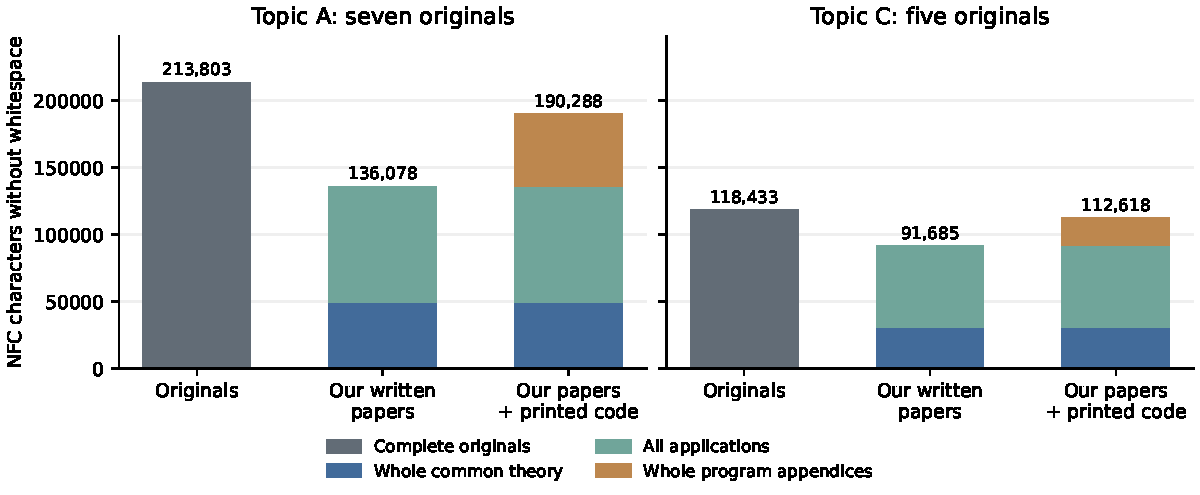
\includegraphics[width=\textwidth]{whole_costs.pdf}\end{center}
Topic A retains its calibrated-selected primary representation. Topic C retains the complete literal rendering of L108 and raw untrimmed PDF extraction for every other source and replacement, including both new common and application documents. The bars use these declared representations; their costs are not pooled into a cross-topic factor.

\begin{center}\small\begin{tabular}{lrrrr}\toprule
 & \multicolumn{2}{c}{Topic A} & \multicolumn{2}{c}{Topic C}\\
NFC unit & Written & With printed code & Written & With printed code\\\midrule
Whitespace tokens & 1.787 & 1.575 & 1.507 & 1.382 \\
Alphanumeric runs & 1.913 & 1.469 & 1.496 & 1.229 \\
Nonspace characters & 1.571 & 1.124 & 1.292 & 1.052 \\
Collapsed characters & 1.610 & 1.191 & 1.329 & 1.103 \\
Collapsed UTF-8 bytes & 1.520 & 1.158 & 1.260 & 1.061 \\
\bottomrule\end{tabular}\end{center}
Exact data preserve raw untrimmed, raw selected and calibrated selected text under NFC and NFKC, in all five units: sixty coordinates and 540 fractions. The twelve application comparisons use the same full acquisition in every coordinate. They do not measure a minimum proof length or establish a mathematical sawtooth pattern by themselves.

\paragraph{Scientific scope and limitations.}
The accepted source contracts and their corrections remain unchanged. L128 retains the qualification that its final proper-quotient claim preserves the same diagram. Frucht's theorem, the small-group classification and exact GAP algorithms are stated outside inputs. L068 includes the corrected construction with its additional incidence condition, the literal counterexample and the qualification of Proposition 3.3; it does not claim that every printed assertion is true. Complete source documents form the numerators because the specified main results have been recovered with these visible qualifications.

The independently accepted additions include all forty-eight pages and all new whole files. Seven delimiter components decoded as whitespace remain visible; the one envelope decoded as seven characters is calibrated as one glyph. Literal line-wrap hooks, extracted graph components and the L108 rendering retain their stated limitations. Full graphics, external proofs, historical software and a complete formalization have unknown costs, not zero.

The three new operational drivers and two Lean files remain separate inventories. The nine added formal declarations verify specific interfaces, not the complete source theorems. Earlier driver and formal inventories are unchanged. No scientific or conjecture credit is added by this numerical update. Previous measurements remain immutable; these new arithmetic, plots and reader require distinct review before admission.
\end{document}
